\documentclass[a4paper,12pt]{article}
\usepackage[left=2cm,top=0cm,right=2cm,bottom=2cm,bindingoffset=0.5cm]{geometry}
\usepackage[english]{babel}
\usepackage{natbib}
\usepackage[utf8x]{inputenc}
\usepackage{graphicx}
\graphicspath{{Report/images/}}
\usepackage{mathtools}
\usepackage{wrapfig}
\usepackage{fancyhdr}
\usepackage{vmargin}
\usepackage{multicol}
\usepackage{url}
\usepackage{hyperref}
\usepackage{textcomp}
% \usepackage[backend=bibtex]{biblatex}
\hypersetup{
	colorlinks = true,
	linkcolor = blue,
	citecolor = red,
	urlcolor = blue
}

\title{Eight Ball Pool}
\author{\textit{kuchbhi}}
\date{October '15}

\makeatletter
\let\thetitle\@title
\let\theauthor\@author
\let\thedate\@date
\makeatother

\pagestyle{fancy}
\fancyhf{}
\rhead{\theauthor}
\lhead{\thetitle}
\cfoot{\thepage}

\begin{document}

\begin{titlepage}
	\centering
    
\includegraphics[scale = 0.09]{Report/images/iitb.jpeg}\\[1.0 cm]	% University Logo
    \textsc{\LARGE IIT Bombay}\\[2.0 cm]				% University Name
	\textsc{\Large CS 251}\\[0.5 cm]				% Course Code
	\textsc{\large Software Systems Lab}\\[0.5 cm]				% Course Name
	\rule{\linewidth}{0.2 mm} \\[0.4 cm]
	{ \huge \bfseries \thetitle}\\
	\rule{\linewidth}{0.2 mm} \\[0.5 cm]
	{\large \thedate}\\[2 cm]

	\renewcommand{\arraystretch}{1.5}
	\begin{table}[!hbt]
	\begin{center}{ \normalsize
	  \begin{tabular*}{\textwidth}{c @{\extracolsep{\fill}} cc}
	 Group & Name & Roll No.  \\
	     \hline
	  & Srajan & 140050017  \\
	 {\huge kuchbhi} & Rishabh & 140050019   \\
	 & Anuj & 140050024  \\
	     \hline
	  \end{tabular*}}
	\end{center}
	\end{table}
 
	\vfill
	
\end{titlepage}

\section{Introduction}
Our project deals with implementing the famous eight ball pool game using C++. We have used a physics simulation engine called Box2D for this purpose. It is a simplified version of the complete game including features like fouls and a complete two player game.

\section{Motivation}
Our hostel has a well maintained pool table with most of the required equipments to play. We often end up playing pool after having our lunch/dinner. We knew the game was all about physics, and as we were supposed to make a project based on a physics simulation engine, we thought why not implement pool?

\section{Insight \& Goals}
\subsection{Introduction to the game}
Eight-ball is played with cue sticks and 16 balls: a cue ball, and 15 object balls consisting of seven striped balls, seven solid-colored balls and the black 8 ball. It is played on a table with six pockets.

After the balls are scattered with a break shot, the players are assigned either the group of solid balls or the stripes once a ball from a particular group is legally pocketed. The ultimate object of the game is to legally pocket the eight ball in a called pocket, which can only be done after all of the balls from a player's assigned group have been cleared from the table.

There are many other intricate rules of the game which will be discussed and implemented in our project.

\subsection{Physics of the game}
\begin{wrapfigure}{r}{0.5\textwidth}
  \begin{center}
    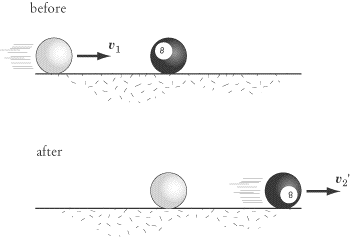
\includegraphics[width=0.48\textwidth]{8ball.png}
  \end{center}
  \caption{1D Collision\cite{1D}} 
\end{wrapfigure}
The whole game revolves around collisions and conservation of momentum. In detail, we look at friction, coefficient of restitution, spin and impulses.
\\\\
In one dimensional motion we define the coefficient of restitution as the velocity of separation divided by the velocity of approach. We'll try to define this formally, and then look at some 2D aspects.
\clearpage
%----------------------------------------------------------------------------%
To solve collisions, we use the coefficient of restitution and the conservation of momentum.

\begin{wrapfigure}{l}{0.48\textwidth}
  \begin{center}
    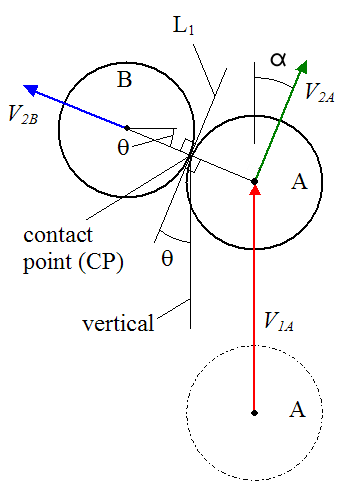
\includegraphics[width=0.44\textwidth]{ball2.png}
  \end{center}
  \vspace{-20pt}
  \caption{2D Collision\cite{2D}}
  \vspace{25pt}
\end{wrapfigure}

In \textbf{one dimensional} motion:

\begin{gather}
e = \frac{v_2' - v_1'}{v_1}\\
mv_2' + mv_1' = mv_1\\
\intertext{where,}
\begin{aligned}
 &e \text{ is the coefficient of restitution}\\
 &v_1 =\text{ is the initial velocity of cue ball}\\
 &v_1' =\text{ is the final velocity of cue ball}\\
 &v_2' =\text{ is the velocity attained by hit ball}
\end{aligned}\notag
\end{gather}
\vspace{0.2cm}

In \textbf{two dimensional} motion:

$$ e = \frac{v_{2B} - v_{2A}sin(\alpha+\theta)}{v_1}$$
$$ mv_{2B}cos\theta = mv_{2A}sin\alpha$$
$$ mv_{2B}sin\theta + mv_{2A}cos\alpha = mv_{1A}$$
\hspace{0.6cm}Typically \cite{data},
$$e_{ball-ball} = 0.92-0.98$$
$$e_{ball-rail} = 0.65-0.85$$

Ofcourse, the balls are also always being acted upon by frictional forces offered by the carpet on the table. Which leads to a constant deceleration.
$$\frac{\mathrm{d} v}{\mathrm{d} t} = - \mu g \approx  -2 m/s^2$$

\subsection{Our proposed goals}
In our Box2D implementation of the game, we will cover all the basic aspects of the game including friction, multiple collisions and pocket detection. Some 3 dimensional aspects of the game like top spin and reverse spin are beyond the scope of this project.\\
The following is a list of objectives that we aim to complete:
\begin{multicols}{2}
\textbf{Core Goals}

\begin{itemize}
  \item Implement all physical interactions
  \item Implement all the standard rules
  \item Set up a two player game
\end{itemize}\columnbreak
\hspace{0.5cm}\textbf{Additional Goals}
\begin{itemize}
  \item Set up an AI to play with
  \item Make a tutorial/beginner mode
  \item Trickshot demonstrations
\end{itemize}
\end{multicols}

\clearpage
%----------------------------------------------------------------------------%

\begin{figure}
	\centering
	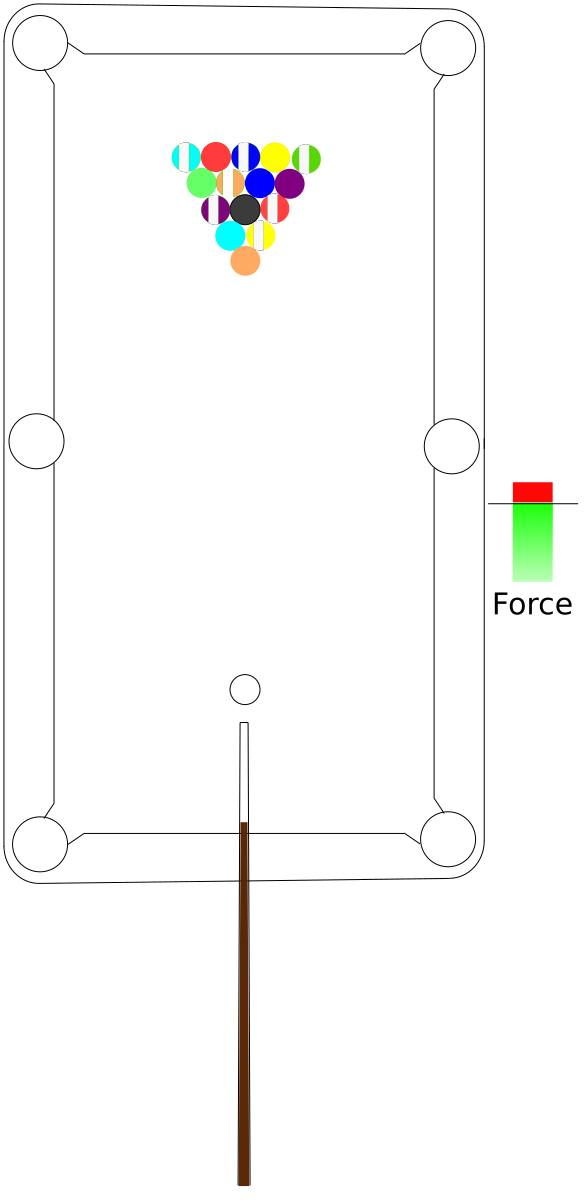
\includegraphics[scale = 0.32]{game.jpg}
	\caption{Stipulated Basic Design}
\end{figure}

\subsubsection{Core Goals:}
Our main aim of the project is get a basic game of pool up and running. Firstly, we have to set up our environment and all the variables correctly. The game will be played with a virtual cue stick which can be rotated around th cue ball with a mouse. It will also have a power setting, basically the speed with which it will hit the cue ball. We will also have to figure out how to detect that a ball has been potted or not, and subsequently remove it from the board if it has.\\

Secondly, we aim at developing a system which will detect all types of fouls which can be encountered while playing the game. After a foul has been committed, we also have to implement the penalty for the foul. This is either an auto-loss for the fouler, or a "ball in hand" for the other player. Thus, by completing a full fledged game, we intend to finish these as our main objectives.
\clearpage


\begin{wrapfigure}{r}{0.52\textwidth}
  \begin{center}
    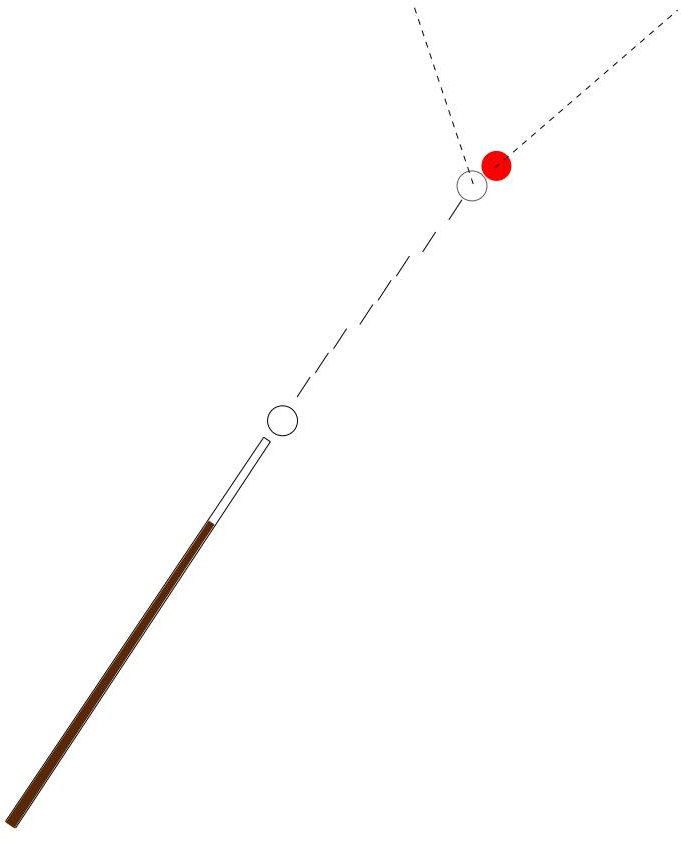
\includegraphics[width=0.5\textwidth]{tut.jpg}
  \end{center}
  \vspace{-20pt}
  \caption{Tutorial Mode}
  \vspace{-140pt}
\end{wrapfigure}

\subsubsection{Tutorial/Beginner mode:}
In this setup, the player will get a "ball guiding system" which will show the trajectory of the cue ball and the ball being hit. This will help new players understand the mechanics of the game, and become more comfortable with the controls.
\subsubsection{Trickshot demonstration:}
Here, the computer will demonstrate "fun to watch" trickshots on the table. (like hitting 3 balls at once) The user will also get the option to try the trickshot himself.

\vspace{3cm}

\section{\cite{Documentation}Our implementation}

\cite{cocos2D}
To start out our project we began, by modifying the given base code to us. We simply, added circular balls and a rectangle to contain the balls initially. We then added circular pockets in the six places. This got us started. We then removed gravity, and set up environment variables like collisions and coefficients of restitution to properly simulate our game. This led us to make the very basic initial model.
Most of this work was done by editing the file dominos.cpp .\\

\cite{cocos2D}
Next, we wanted to add the ability of the user to actually interact with the balls. So, we started working on the implementation of the pool stick and how the mouse will control this stick. We got the stick to rotate around the cue ball, and the user must pull the stick and let go to actually hit it. We were satisfied with how this mechanism was working. All this work was done by modifying the mouse\_up , mouse\_down and mouse\_move functions.\\

\cite{b2ContactListener} \cite{iforce2D}
After this we started thinking about how to delete balls, when they got in contact with the pocket. We knew we couldn't do this as it happens in the real game, so we decided to erase the ball, if it came in contact with the pocket circles. We got this working using the b2ContactListener class. We then worked on differentiating the balls by colouring them up, and also looked at the aesthetic point of view of the game. After this the front end display was set up, showing the score and other details about the progress of the game.\\

We now needed to work about the backend of keeping the score and the foul system. The basic rules of the game were implemented, like the first touch rule, or the cue ball being pocketed foul. The opponent of the player who committed the foul gets two turns in succession. All this helped us shape the flow control of the whole game.\\


Unfortunately, we had run out of time, and also had to focus on our other project, the Web App. This resulted in us not being able to finish the 
other goals we had in mind. We have a basic GUI pool game for two players running, but we could not fulfill any of our additional goals.\\

\section{Demo}
You can find a video\cite{software} demonstrating the project \href{https://www.youtube.com/watch?v=ccL42N-W_bU}{here}.\\
Also, the project webpage\cite{template} can be accessed at the following \href{http://www.cse.iitb.ac.in/~rishabhagarwal/links/web/index.html}{link}\\

\begin{figure}
	\centering
	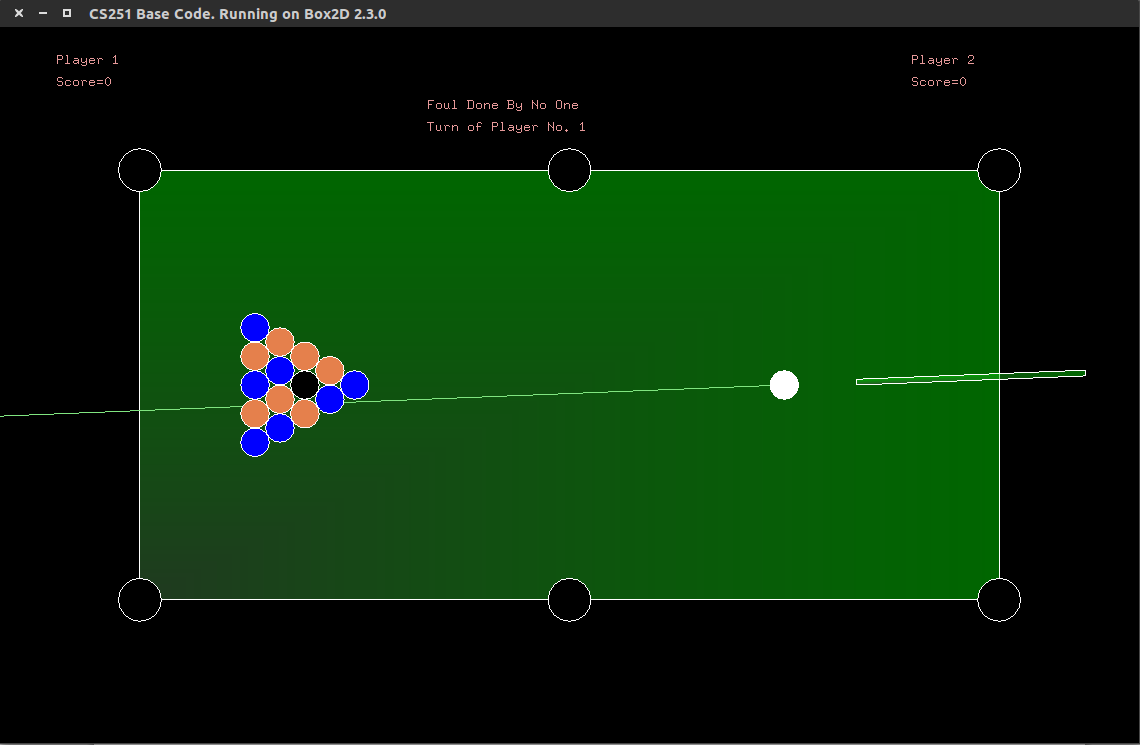
\includegraphics[scale = 0.35]{Report/images/main.png}
	\caption{Basic Design}
\end{figure}
\clearpage

\section{\cite{gprof}Profiling} 
The code profiling was done using gprof and the graphviz package. 
In our case, Profiling didn't help much to optimize the code as the most of time was taken inside the inbuilt Box2d functions. 

The call graph when library is compiled using debug version and without using optimisation flags  before making any changes in the code is
\begin{figure}[h]
  \centering
  
\includegraphics[scale = 0.04]{Report/images/call_graph.png}
  \caption{Debug Version}
\end{figure}
There are a lot of functions in the call graph. Most of the code written by us was optimized as the most time was taken by the inbuilt functions in box2D implementations.Almost all the functions in the call graph directly or indirectly calls the function b2Vec2::b2Vec2(float, float)\
The top 5 functions on the basis of total running time of the program used by this function are:-
\begin{enumerate}
\item operator*(float, b2Vec2 const\&)
\item operator+(b2Vec2 const\&, b2Vec2 const\&)
\item debug\_draw\_t::DrawSolidCircle(b2Vec2 const\&, float, b2Vec2 const\&,\\
 b2Color const\&)
\item b2Vec2::b2Vec2(float, float)
\item debug\_draw\_t::DrawString(int, int, char const*, ...)
\end{enumerate}

Though the top two functions that are in green color in the call-graph are b2World::DrawShape(b2Fixture*, b2Transform const\&, b2Color const\&)
and debug\_draw\_t::DrawSolidCircle(b2Vec2 const\&, float, b2Vec2 const\&, b2Color const\&).

The call graph when library is compiled using Release version and using optimisation flags before making any changes in the code is
\begin{figure}[h]
  \centering
  
\includegraphics[scale = 0.04]{Report/images/call_graphRelease.png}
  \caption{Release Version}
\end{figure}

It is similar to what one obtains using the debug version, however since function is optimized the time spent decreases for each function and also 
the \% spent in each function decreases.
The top 5 functions on the basis of total running time of the program used by this function are:-
\begin{enumerate}
\item debug\_draw\_t::DrawSolidCircle(b2Vec2 const\&, float, b2Vec2 const\&,\\ b2Color const\&)
\item debug\_draw\_t::DrawString(int, int, char const*, ...)
\item b2World::Solve(b2TimeStep const\&)
\item b2World::SolveTOI(b2TimeStep const\&)
\item void b2DynamicTree::Query\textlangle{}b2BroadPhase\textrangle{}(b2BroadPhase*,\\b2AABB const\&) const
\end{enumerate}

Only the second function in the call-graph i.e  cs251::callbacks\_t::display\_cb() which contains a function 
cs251::base\_sim\_t::step(cs251::settings\_t*) includes a function update\_turn() implemented by us takes about 1\% of total time.


The call graph of the Original Base code when library is compiled using release version and using optimisation looks like 
\begin{figure}[h]
  \centering
  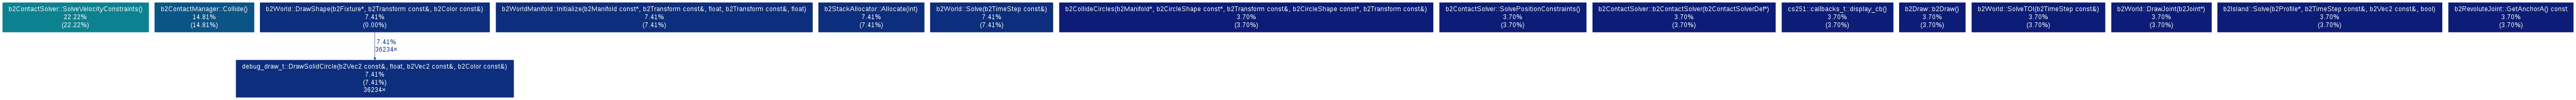
\includegraphics[scale = 0.08]{Report/images/call_graphOriginal.png}
  \caption{Debug Version}
\end{figure}

This is quite different in terms of the top functions as we changed the dominos.cpp file completely and added a pool table, edges and multiple 
balls and the game involves their interaction.
The top 5 functions are:-
\begin{enumerate}
\item b2ContactSolver::SolveVelocityConstraints()
\item b2ContactManager::Collide()
\item debug\_draw\_t::DrawSolidCircle(b2Vec2 const\&, float, b2Vec2 const\&,\\
      b2Color const\&)
\item b2WorldManifold::Initialize(b2Manifold const*,
      b2Transform const\&,\\ float,b2Transform const\&, float)
\item b2StackAllocator::Allocate(int)
\end{enumerate}

The top functions are different because our interface includes drawing a lot of balls and updating them on the screen which involves
debug\_draw\_t::DrawSolidCircle(\\b2Vec2 const\&, float, b2Vec2 const\&, b2Color const\&)and also keeping track of the score and other
variables for which the debug\_draw\_t::DrawString(int, int,
char const*, ...) is called multiple times. 

\clearpage

\section{Work distribution}
We started discussion about what to implement as a Rube-Goldberg machine in mid-August. We decided not to implement the standard machine, rather make a game using the physics engine. We got confirmation from Prof. Sharat and started working on the project mid-September.\\

Though the work of each team member was closesly interlinked, we divided the work as follows:
\begin{itemize}
  
  \item Srajan Garg (140050017): 
  \vspace{-0.2cm}
  \begin{itemize}
  	\setlength{\itemsep}{-0.1cm}
  	\item Discussion of ideas and how they were to be implemented
  	\item Coding of the base strucutre of the game, the balls, table and pockets
  	\item Setting up environment variables like no gravity, restitution and friction
  	\item Coding up the contact listener to implement the pocketing of balls
  	\item Making of the report
  \end{itemize}
  \vspace{-0.2cm}

  \item Rishabh Agarwal (140050019):
  \vspace{-0.2cm} 
  \begin{itemize}
  	\setlength{\itemsep}{-0.1cm}
  	\item Discussion of how the code is going to be structured
  	\item Coding up aesthetic aspects of the game, like ball colours and the table
  	\item Set up the frontend interface and implemented the turn-based mechanism
  	\item Implemented the foul play and rules of the game by improving upon contactListener and Step function 
    \item Doxygen documentation of all the changes in the base code
    \item Gprof Profiling and optimization of the code and adding its details to report 
  	\item Making of the informative video on the project
  \end{itemize}
  \vspace{-0.2cm}

  \item Anuj Mittal (140050024): 
  \vspace{-0.2cm}
  \begin{itemize}
  	\setlength{\itemsep}{-0.1cm}
  	\item Discussion about the flow control of the program
  	\item Coded up the implpementation of cue stick
  	\item Integrated mouse support with stick, to 'rotate' and 'pull' it
  	\item Discussed implementation of fouls and improved on some functionality of game
  	\item Making of the webpage related to the project
  \end{itemize}
  \vspace{-0.2cm}

\end{itemize}

\section{Conclusion}
All in all it was a great learning experience. We learned how to work in a team. One of the most important aspects of the project was to work, while using git. This helped us to understand version control and why it is essential for any project. More importantly we got a feel of how large organisations use repositories for storing codebases. We got to know how a distributed system works. This helped us to collaborate our work, and spend our time productively.\\

We also learnt how to use other poeples' projects and codebases. We learnt how a distributable version of a software is made. Box2D helped us understand te inner implementations of how a large engine works. Learning about CMake and makefiles was also a good experience, and we realized how important they are for any large scale project.


\section{Honour Code}

I, Srajan Garg, pledge on our honour that I have not given or received any unauthorized assistance on this project or any previous task.\\ \\
I, Rishabh Agarwal, pledge on our honour that I have not given or received any unauthorized assistance on this project or any previous task.\\ \\ 
I, Anuj Mittal, pledge on our honour that I have not given or received any unauthorized assistance on this project or any previous task.\\ \\

\begin{small}
\bibliography{report}
\bibliographystyle{unsrt}
\end{small}
\end{document}
\grid
\grid
\grid